\externaldocument{MachineLearning.tex}
\chapter{Evaluation of OCR}
\label{sec:Evaluation of OCR}
Here is an evaluation of random forest when used for character recognition and point pair features. During training there are a number of different parameters which can have high significance for the resulting classifier. When using the classifier for testing the amount of overlap of the tile is also of hight importance. In the end of the chapter the training with point pair features are also compared with two-rectangle features. In each step in the evaluation there is a measure of the accuracy and the processing time.

\section{Evaluation of training}
\label{sec:Evaluation of training}
The system for OCR are using two different classifier, one for separation of background and characters and one for classification of the individual character. Hence the evaluation has been done for both classifiers separately.
 
\subsection{Classifier for individual characters}
\label{sec:Classifier for individual characters}
Here follows an evaluation for the training of the classifier 2 which is used for classification of individual characters. The classifier has been trained with different amount of features, different number of trees and different amount of training data. The evaluation has been made with test data which is similar to the training data, i.e. the statistical properties of the translation and rotation of the characters are the same as for the training. The amount of training data is much less then in the final classifier, this is because all the trainings would take too much time otherwise. The evaluation will all the same give an understanding how the different parameters affect the result. 

The training has been done for two different amount of training data. For each of these there are three individual tables where the number of point pairs has been compared to the amount of trees in the forest. The fires table gives the average amount of true detection in percent. 

In the second table the average majority votes in percent are given, i.e. how big is the amount of trees that made the same prediction as the final result. The upper value in each cell is the majority vote when the prediction was correct, and the lower is the majority vote when the prediction was incorrect. 

In the third table gives the average time for each character, i.e. the time to calculate the features and make a prediction.

The accuracy seems to vary slightly when running a test several times, although the numbers in the tables gives a good hint of the performance.

First the result for training with 4100 training data is presented.
 
\begin{table}[H]
\begin{center}
     \begin{tabular}{| l | l | l | l | l | l | }
     \hline
     no. of point pairs & 1 tree & 20 trees & 50 trees & 100 trees & 500 trees \\ \hline
   	 100 & 33\% & 78\% & 80\% & 84\% & 85\% 	\\ \hline
     500 & 37\% & 82\% & 88\% & 91\% & 92\%	\\ \hline
     1000 & 40\% & 81\% & 88\% & 91\% & 91\% \\ \hline
     10000 & 37\% & 84\% & 87\% & 92\% & 91\%	\\ \hline
     20000 & 38\% & 83\% & 88\% & 90\% & 93\% 	\\ \hline
     \end{tabular}
\end{center}
\caption{The amount of true detection in percent for classifier trained with different numbers of point pairs and different amount of trees using 4100 training data}
\end{table}

\begin{table}[H]
\begin{center}
     \begin{tabular}{| l | p{1.2cm} | p{1.2cm} | p{1.2cm} | l | l | }
     \hline
     no. of point pairs & 1 tree & 20 trees & 50 trees & 100 trees & 500 trees \\ \hline
   	 100 & 100\% \newline 100\% & 43\% \newline 30\% & 40\% \newline 30\% & \newline & \newline 	\\ \hline
     500 & 100\% \newline 100\% & 44\% \newline 29\% & 43\% \newline 27\% & \newline & \newline	\\ \hline
     1000 & 100\% \newline 100\% & 44\% \newline 30\% & 42\% \newline 28\% & \newline & \newline \\ \hline
     10000 & 100\% \newline 100\% & 45\% \newline 26\% & 43\% \newline 28\% & \newline & \newline 	\\ \hline
     20000 & 100\% \newline 100\% & 44\% \newline 27\% & 43\% \newline 26\% & \newline & \newline	\\ \hline
     \end{tabular}
\end{center}
\caption{The average value in percent for the majority vote for true and false detections respectively. Classifier has been trained with different numbers of point pairs and different amount of trees using 4100 training data}
\label{table:mojorityVote1}
\end{table}


\begin{table}[H]
\begin{center}
     \begin{tabular}{| l | l | l | l | l | l | }
     \hline
     no. of point pairs & 1 tree & 20 trees & 50 trees & 100 trees & 500 trees \\ \hline
   	 100 & 0.004 ms & 0.015 ms & 0.03 ms & 0.06 ms & 0.62 ms \\ \hline
     500 & 0.012 ms & 0.024 ms & 0.04 ms & 0.07 ms & 0.62 ms\\ \hline
     1000 & 0.021 ms & 0.034 ms & 0.05 ms & 0.08 ms & 0.62 ms \\ \hline
     10000 & 0.19 ms & 0.21 ms & 0.23 ms & 0.26 ms & 0.81 ms \\ \hline
     20000 & 0.37 ms & 0.38 ms & 0.41 ms & 0.47 ms & 1.01 ms	\\ \hline
     \end{tabular}
\end{center}
\caption{Average time in ms for classifier trained with different numbers of point pairs and different amount of trees using 4100 training data}
\end{table}

Here is the result for training with 16400 training data using the same parameters as above.

\begin{table}[H]
\begin{center}
     \begin{tabular}{| l | l | l | l | l | l | }
     \hline
     no. of point pairs & 1 tree & 20 trees & 50 trees & 100 trees & 500 trees \\ \hline
   	 100 & 41\% & & & 90\% & 92\%  	\\ \hline
     500 & 53\% & & & 94\% & 96\%  	\\ \hline
     1000 & 52\% & & & 95\% & 95\%  	\\ \hline
     10000 & 56\% & & & 95\% & 96\% 	\\ \hline
     20000 & 49\% & & & 95\% & 	\\ \hline
     \end{tabular}
\end{center}
\caption{The amount of true detection in percent for classifier trained with different numbers of point pairs and different amount of trees using 16400 training data}
\end{table}

\begin{table}[H]
\begin{center}
     \begin{tabular}{| l | p{1.2cm} | l | l | l | l | }
     \hline
     no. of point pairs & 1 tree & 20 trees & 50 trees & 100 trees & 500 trees \\ \hline
   	 100 & 100\% \newline 100\% & & & & 	\\ \hline
     500 & 100\% \newline 100\% & & & &  	\\ \hline
     1000 & 100\% \newline 100\% & & & &  \\ \hline
     10000 & 100\% \newline 100\% & & & &  	\\ \hline
     20000 & 100\% \newline 100\% & & & &   	\\ \hline
     \end{tabular}
\end{center}
\caption{The average value in percent for the majority vote for true and false detections respectively. Classifier has been trained with different numbers of point pairs and different amount of trees using 16400 training data}
\label{table:mojorityVote2}
\end{table}



\begin{table}[H]
\begin{center}
     \begin{tabular}{| l | l | l | l | l | l | }
     \hline
     no. of point pairs & 1 tree & 20 trees & 50 trees & 100 trees & 500 trees \\ \hline
   	 100 & 0.004 & & & 0.067 & 0.68  	\\ \hline
     500 & 0.015 & & & 0.074 & 0.68  	\\ \hline
     1000 & 0.023 & & & 0.084 & 0.67  	\\ \hline
     10000 & 0.18 & & & 0.27 & 0.89 	\\ \hline
     20000 & 0.37 & & & 0.46 & 	\\ \hline
     \end{tabular}
\end{center}
\caption{Average time in ms for classifier trained with different numbers of point pairs and different amount of trees using 16400 training data}
\end{table}

\subsection{Classifier for separation of characters and background}
\label{sec:Classifier for separation of characters and background}
Classifier 1 which is used for separation of characters and background has been evaluated with different number of trees, different amount of training data and different number of features. The amount of true and false samples in the training dataset is approximately the same.

\begin{table}[H]
\begin{center}
     \begin{tabular}{| l | l | l | l | l | l | }
     \hline
     training data & 1 tree & 20 trees & 50 trees & 100 trees & 500 trees \\ \hline
     1042 & 83\% & 84\% & 85\% & 88\% & 92\% 		\\ \hline
   	 10420 & 89\% & 97\% & 91\% & 95\% & 93\%  	\\ \hline
     20840 & 92\% & 93\% & 92\% & 94\% & 95\% 		\\ \hline

     \end{tabular}
\end{center}
\caption{The amount of true detection in percent for classifier trained with different number of trees and different amount of training data}
\end{table}

\begin{table}[H]
\begin{center}
     \begin{tabular}{| l | l | l | l | l | l | }
     \hline
     training data & 1 tree & 20 trees & 50 trees & 100 trees & 500 trees \\ \hline
     1042 & 11663\% & 1087\% & 651\% & 643\% & 411\% 		\\ \hline
   	 10420 & 6074\% & 258\% & 96\% & 52\% & 11\%  	\\ \hline
     20840 & 4202\% & 356\% & 170\% & 333\% & 252\% 		\\ \hline

     \end{tabular}
\end{center}
\caption{The amount of true detection in percent for classifier trained with different number of trees and different amount of training data}
\end{table}

\begin{table}[H]
\begin{center}
     \begin{tabular}{| l | p{1.2cm} | p{1.2cm} | p{1.2cm} | p{1.2cm} | p{1.2cm} | }
     \hline
     training data & 1 tree & 20 trees & 50 trees & 100 trees & 500 trees \\ \hline
     1042 & 100\% \newline 100\% & 93\% \newline 80\% & 93\% \newline 72\% & 93\% \newline 85\% & 91\% \newline 68\% 		\\ \hline
   	 10420 & 100\% \newline 100\% & 96\% \newline 69\% & 96\% \newline 69\% & 97\% \newline 71\% & 97\% \newline 79\% 	\\ \hline
     20840 & 100\% \newline 100\% & 93\% \newline 74\% & 92\% \newline 67\% & 94\% \newline 65\% & 95\% \newline 65\% 		\\ \hline

     \end{tabular}
\end{center}
\caption{The average value in percent for the majority vote for true and false detections respectively. Classifier has been trained with different numbers of trees and different amount of training data}
\label{table:mojorityVote3}
\end{table}

\begin{table}[H]
\begin{center}
     \begin{tabular}{| l | l | l | l | l | l | }
     \hline
     training data & 1 tree & 20 trees & 50 trees & 100 trees & 500 trees \\ \hline
     1042 & 0.07 ms & 0.06 ms & 0.08 ms & 0.094 ms & 0.24 ms		\\ \hline
   	 10420 & 0.06 ms & 0.07 ms & 0.07 ms & 0.1 ms & 0.35 ms	\\ \hline
     20840 & 0.07 ms & 0.06 ms & 0.09 ms & 0.12 ms & 0.43 ms  		\\ \hline

     \end{tabular}
\end{center}
\caption{Average time in ms for classifier trained with different numbers of trees and different amount of training data}
\end{table}

\section{Other training parameters for Random forest}
\label{sec:Other training parameters for Random forest}
In the random forest algorithm there are some other parameter values that can be altered.
\begin{center}
\begin{itemize}
	\item The maximum depth of the trees
	\item The minimum number of samples in a leaf node
	\item The number of active variable in a split
	\item The type of the termination criteria
\end{itemize}
\end{center}
There has not been any thorough evaluation of these parameters. The maximum depth of the trees determines how deep a tree can get before it stops growing. This parameter has here been set to 10. In figure \ref{treeplot} is an illustration of a randomly chosen tree. As one can see, a maximum depth of 10 should be more than enough for a problem with 36 different classes.

\begin{figure}[H]
\centering
	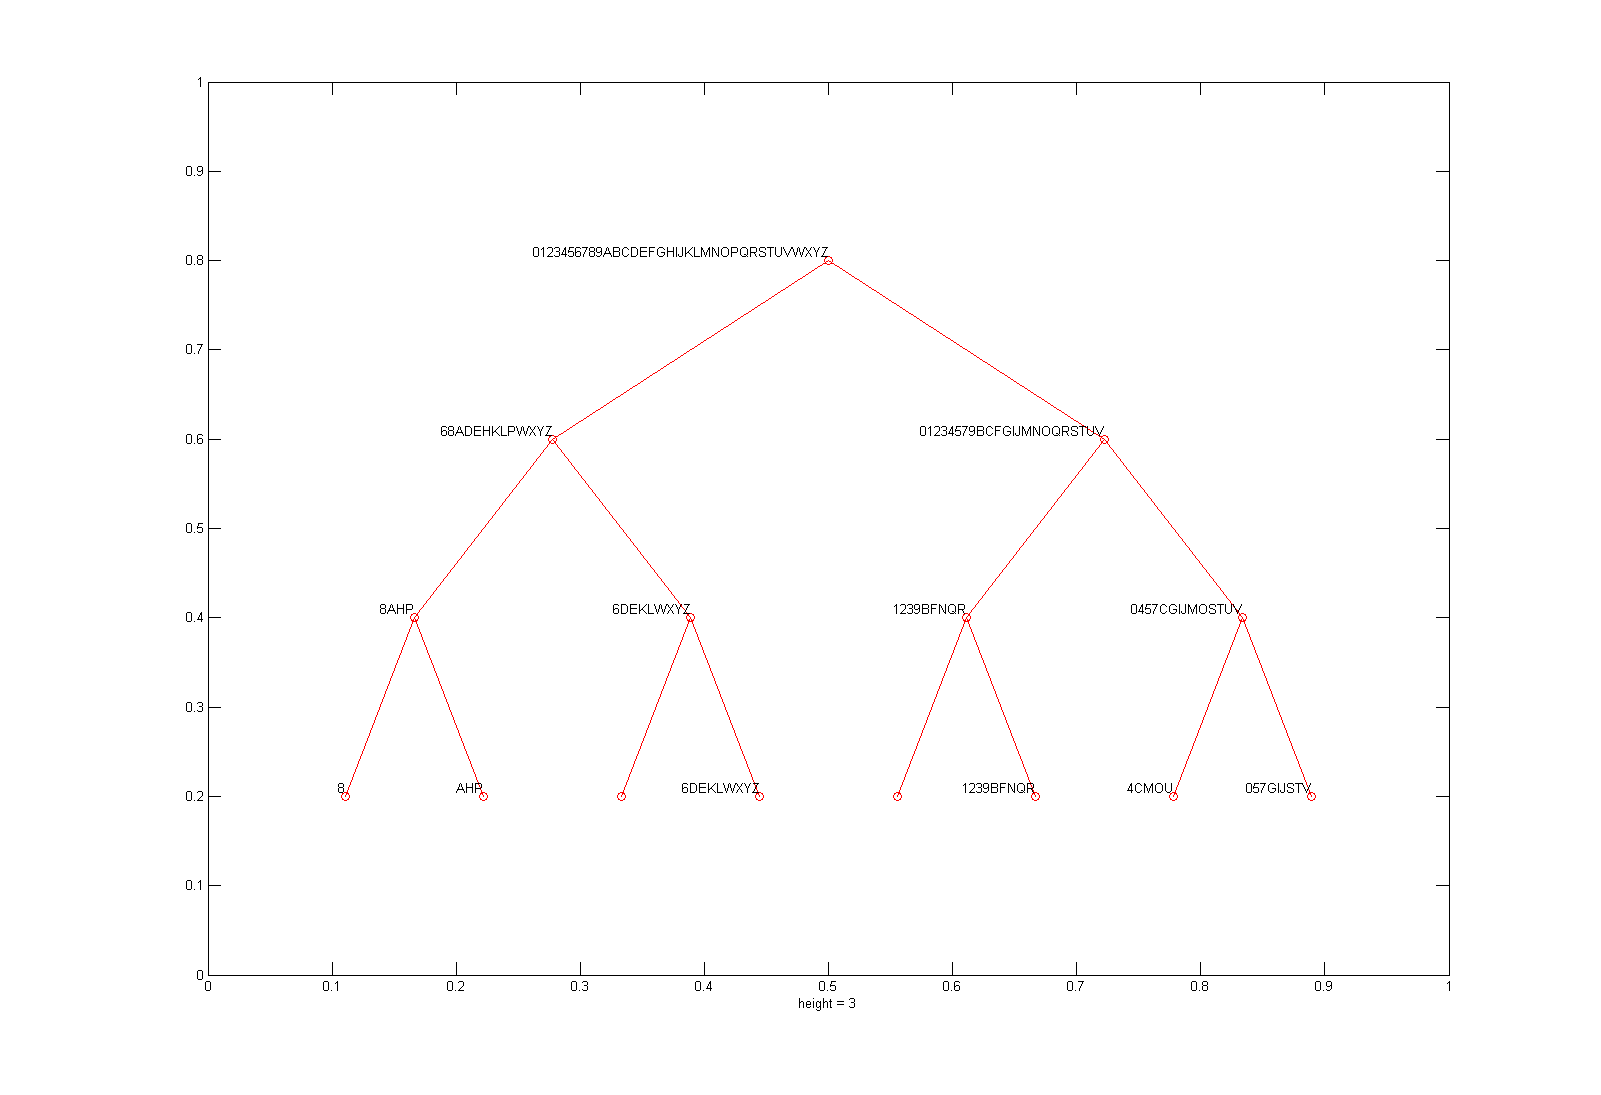
\includegraphics[scale=0.3]{treeplot}
	\caption{Illustration of the 4 upper levels in one of trees from a classification forest}
	\label{treeplot}
\end{figure}

The minimum number of samples in a leaf node refers to $N$ in equation  \ref{eq:Einf}. This is the minimum number of samples in a node which is required for it to be split. This parameter has been set to 5 but some higher values has also been tried. By increasing it the training should be faster but it does not seem to have any significant effect during testing.

The number of active variables in a split determines how many features each split will chose randomly. By altering this parameter it is possible to control the randomness of the forest. A high parameter value will lead to more correlated trees. A normal value for this parameter is the square root of the total number of features, this is also what has been used here.

Also it is possible to chose what type of termination criteria to use, i.e. when will the training stop. The most common is to terminate the training when the number of trees has reached a certain value. This is the criteria that has been used here.
\section{Result for some test images}
\label{sec:Result for some test images}
%There are not really any easy way to evaluate the classifier when used to detect characters in real images. The only way is to first label the images manually and then when using the classifier evaluate the accuracy and the speed. The accuracy is measured in the following way:
%
%\begin{center}
%\begin{itemize}
%\item The amount of true detection in percent
%\item The number of false detections
%\end{itemize}
%\end{center}

When the classifier is used to detect characters in an images a tile of the size 54 times 64 is moved over the image. This can be done with different amount of overlap, i.e. how much two adjacent tiles overlap each other. The amount of overlap that is used will affect the result significantly, both when it comes to accuracy and speed. However it is obvious that the tiles need to overlap each other a lot. Here the images have been tested with two different amount of overlap, 8 and 16.

The classifiers used here have been trained by first studying the result from section \ref{sec:Evaluation of training}. 

From these results the training for classifier 1 was done with the following settings:
\begin{center}
\begin{itemize}
\item Amount of training data: 49800
\item Number of trees: 50
\end{itemize}
\end{center} 
The training of classifier 2 has been trained with the following settings:
\begin{center}
\begin{itemize}
\item Amount of training data: 46000
\item Number of trees: 100
\item Number of point pairs: 500
\end{itemize} 
\end{center}

The thresholds for the amount of trees in the majority vote is based on the result in table \ref{table:mojorityVote1}, \ref{table:mojorityVote2} and \ref{table:mojorityVote3}. For classifier 1 the threshold is set to 0.95 and for classifier 2 the threshold is set to 0.3.

The first test image, \ref{im7}, is just a printed page consisting of some letters and digits in different sizes.

\begin{figure}[H]
\centering
	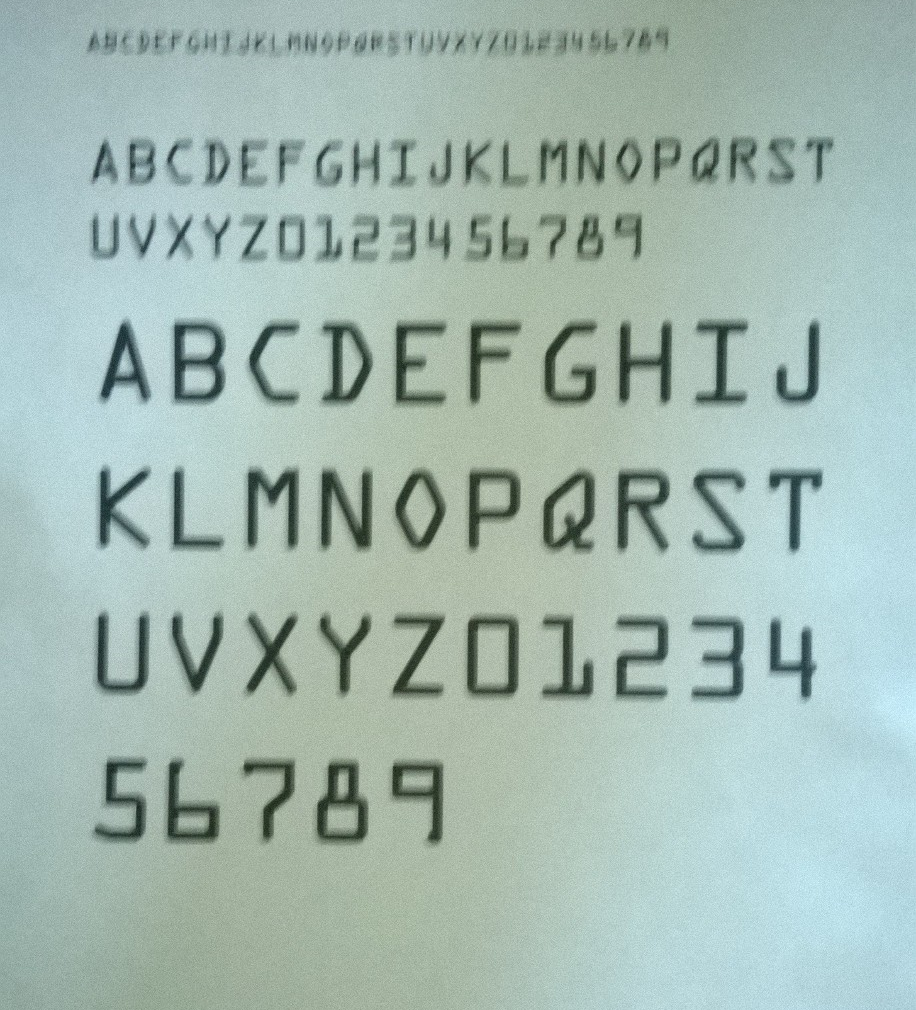
\includegraphics[scale=0.4]{im7}
	\caption{Test image 1 for OCR}
	\label{im7}
\end{figure}

In figure \ref{im7res1} and \ref{im7res2} are the result for image 1 when trying to detected the largest characters. First is the result from the first classifier and then the result from the second classifier.

\begin{figure}[H]
\centering
	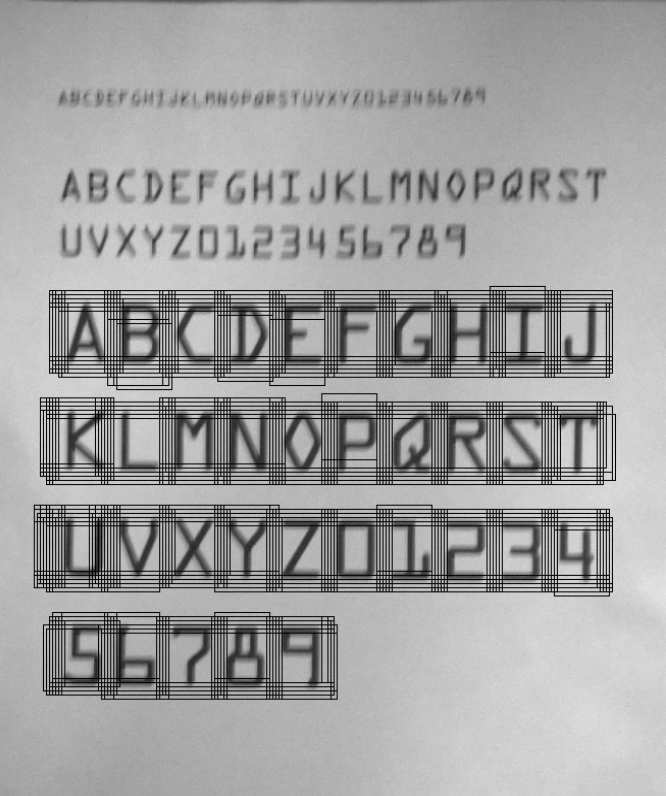
\includegraphics[scale=0.5]{im7Class1}
	\caption{Result after classifier 1 has been applied to image 1}
	\label{im7res1}
\end{figure}

\begin{figure}[H]
\centering
	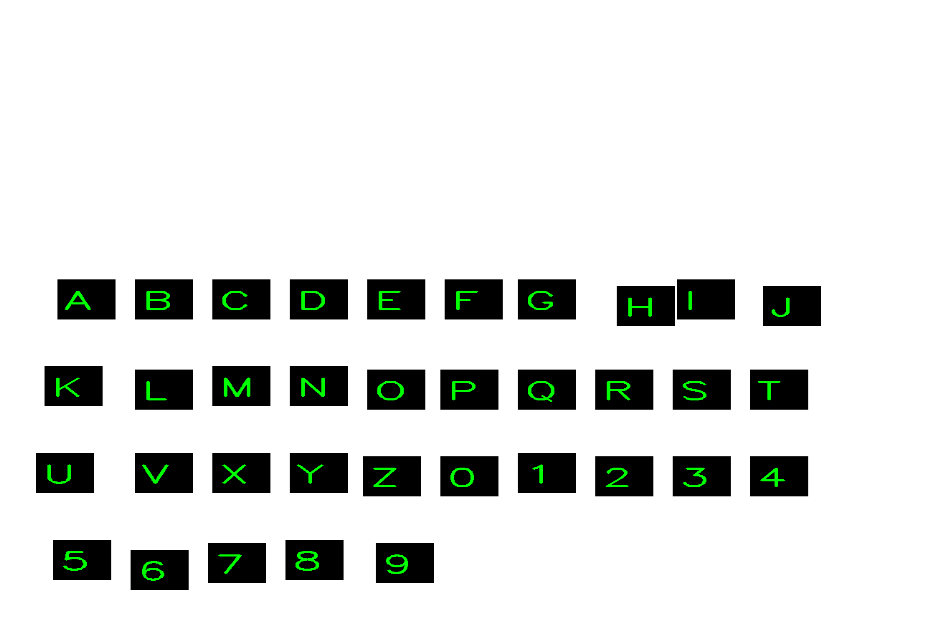
\includegraphics[scale=0.5]{im7Class2}
	\caption{Result after classifier 2 has been applied to image 1}
	\label{im7res2}
\end{figure}

The second, \ref{im22} illustrates a typical example from a real application. The part of the image containing the text of interest has been zoomed in. Still there are a lot of other details and characters which are not supposed to be detected. Also among the desired characters there are two characters that have not been used during training.

\begin{figure}[H]
\centering
	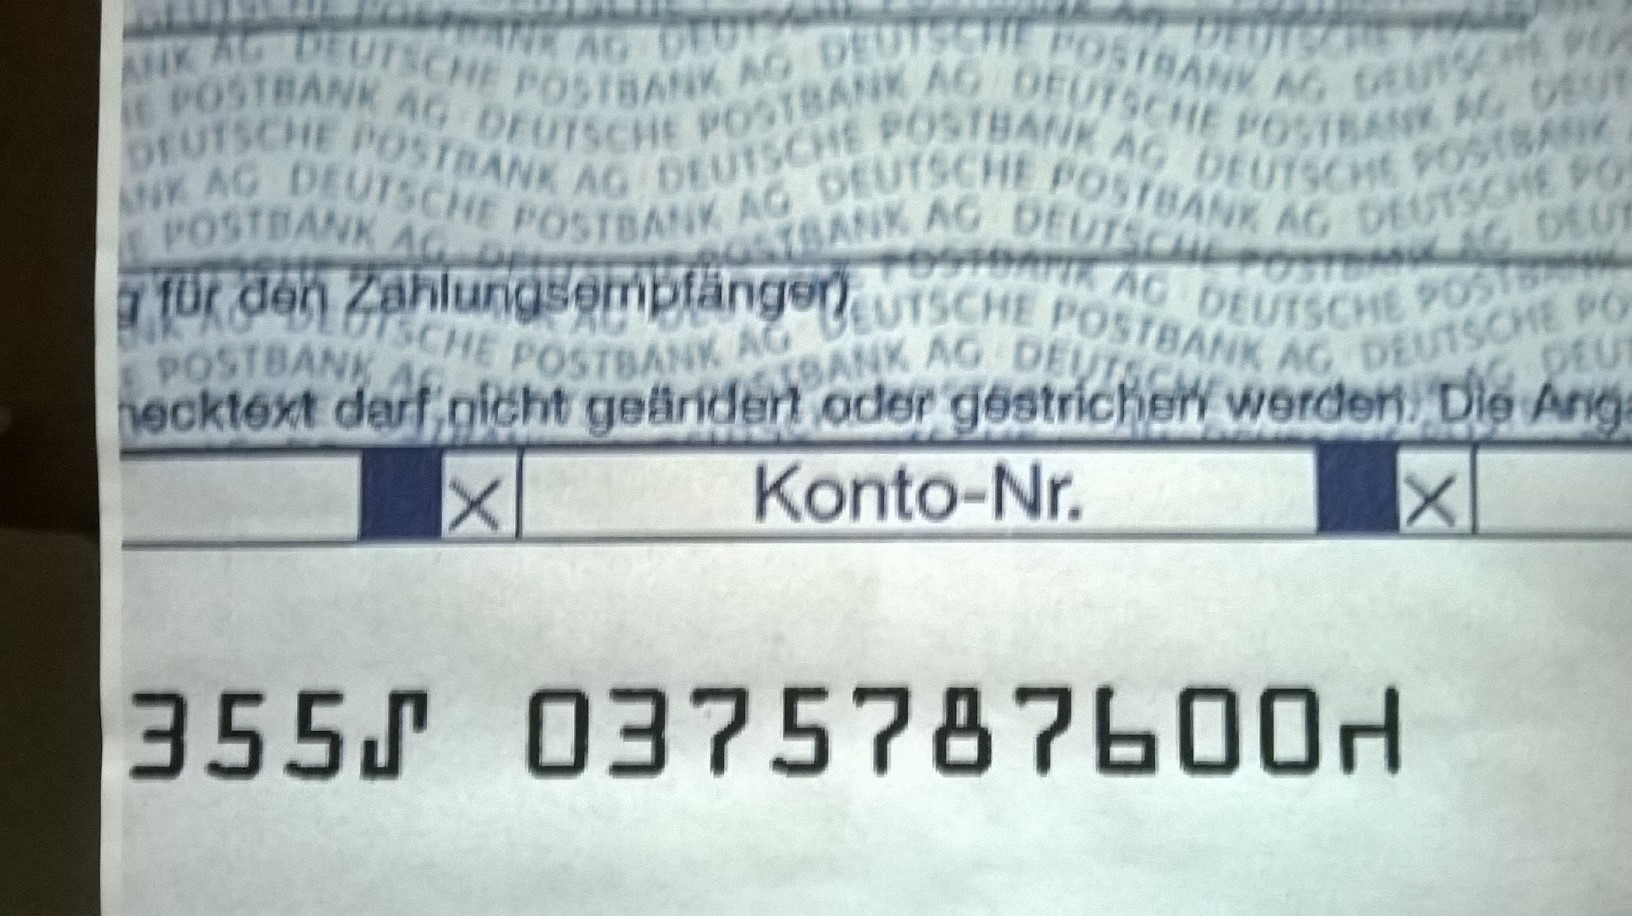
\includegraphics[scale=0.2]{im22}
	\caption{Test image 2 for OCR}
	\label{im22}
\end{figure}

Here is the result for image 2 for tiles with overlap 16.

\begin{figure}[H]
\centering
	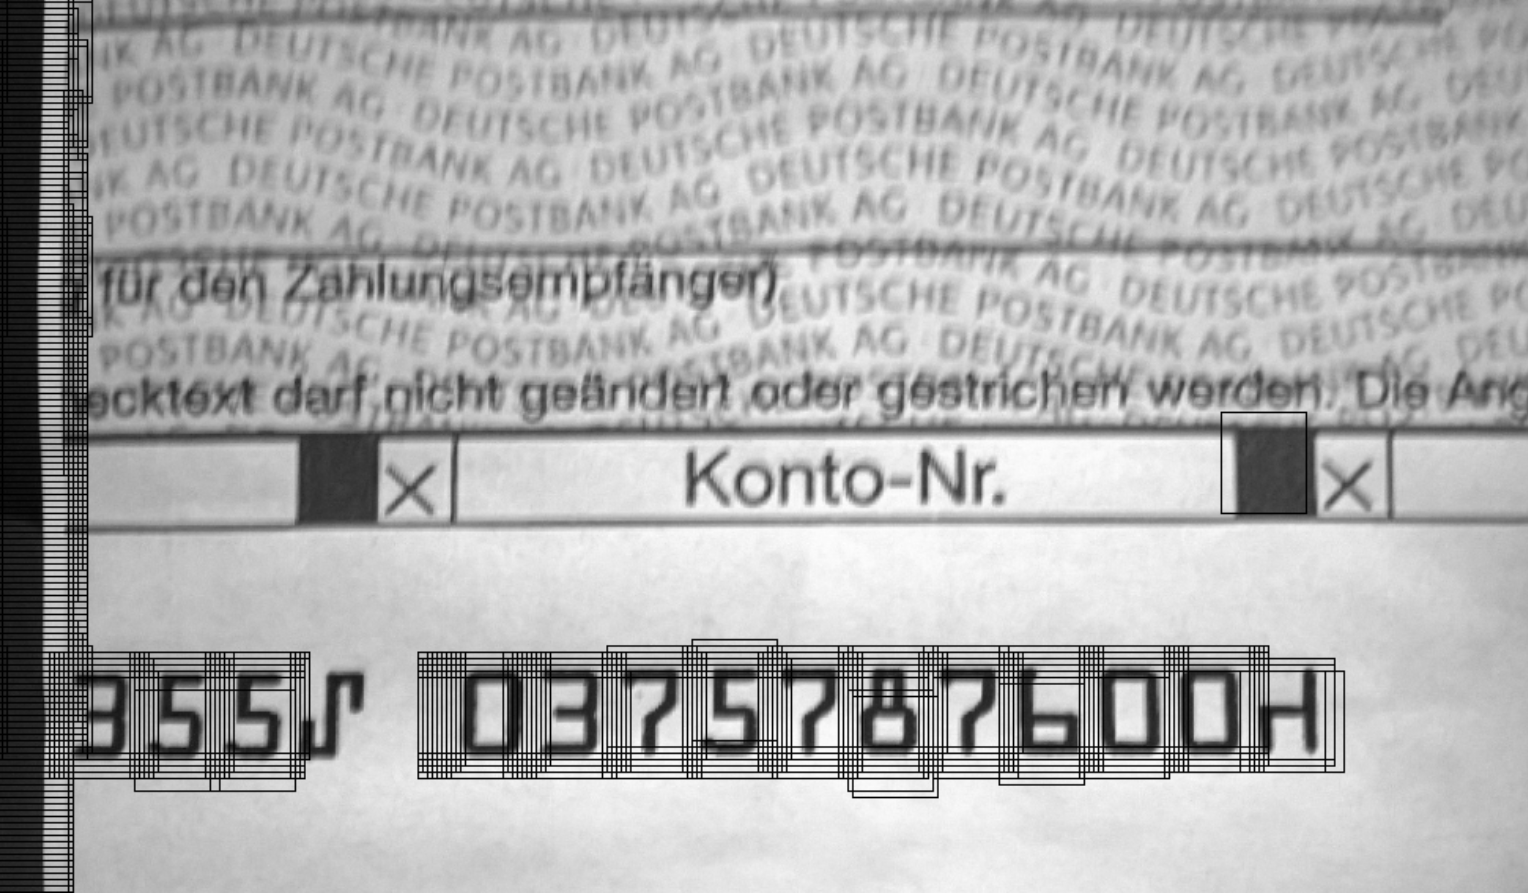
\includegraphics[scale=0.3]{im22Class1}
	\caption{Result after classifier 1 has been applied to image 2}
	\label{im22res1}
\end{figure}

\begin{figure}[H]
\centering
	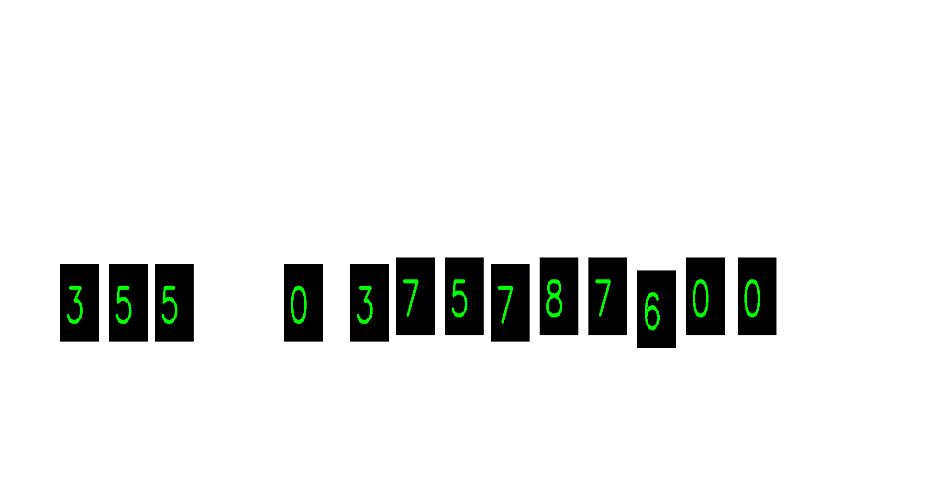
\includegraphics[scale=0.5]{im22Class2}
	\caption{Result after classifier 2 has been applied to image 2}
	\label{im22res2}
\end{figure}

Table \ref{table:result test} gives the result for the two images with different amount of overlap.

\begin{table}[H]
\begin{center}
     \begin{tabular}{| l | l | | l |}
     \hline
       & overlap 8 & overlap 16 \\ \hline
     image 1 & 0.35 s & 1.48 s\\ \hline
     image 2 & 0.19 s & 0.6 s \\ \hline
     \end{tabular}
\end{center}
\label{table:result test}
\caption{Processing time for two different images with overlap 8 and overlap 16}
\end{table}

\subsection{Cases when the system fails}
\label{sec:Cases when the system fails}
One case which the system does not seem to be able to handle is when there are other characters in the image which are bigger then the characters of interest. When trying to detect the smaller characters in image \ref{im7} the first classifier finds many false detections. This is illustrated in figure \ref{im7fail}. In this case classifier 2 will fail completely.

\begin{figure}[H]
\centering
	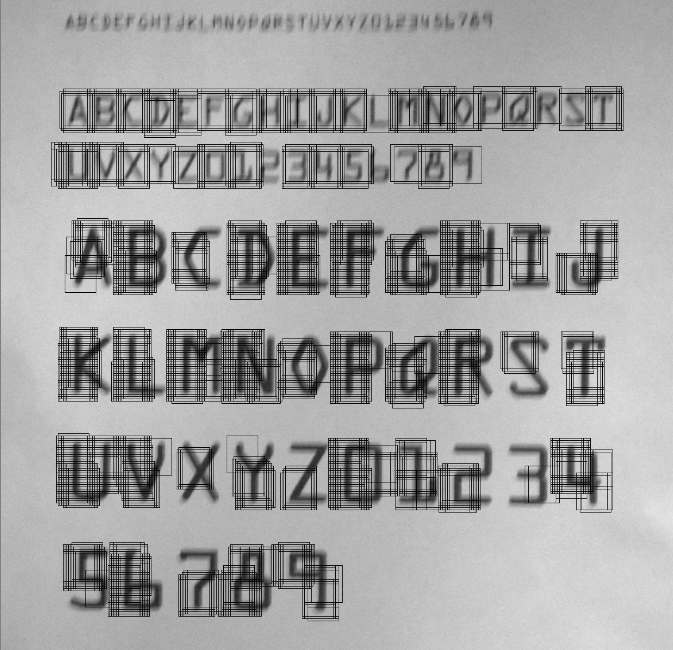
\includegraphics[scale=0.5]{im7fail}
	\caption{Result after classifier 1 has been applied to the smaller characters in test image 1}
	\label{im7fail}
\end{figure}
 
The system will also fail if the characters in the image has an appearance which has not been used during training. During training the character samples are rotated randomly with some degree. If the image contains characters which are rotated more than the training samples it will lead to a bad result. In figure \ref{im7fail2} and \ref{im7fail3} are the results when figure \ref{im7} has been rotated too much.

\begin{figure}[H]
\centering
	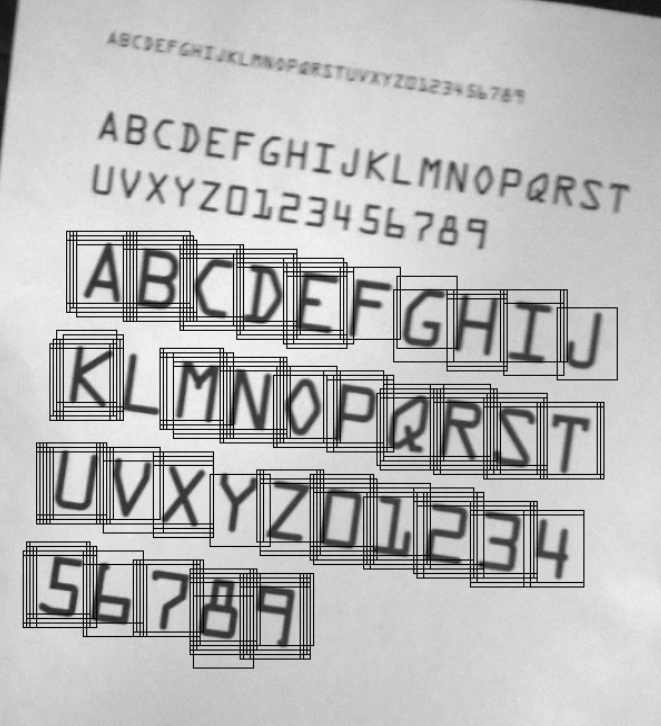
\includegraphics[scale=0.5]{im7fail3}
	\caption{Result after classifier 1 has been applied to a rotated version of test image 1}
	\label{im7fail2}
\end{figure}

\begin{figure}[H]
\centering
	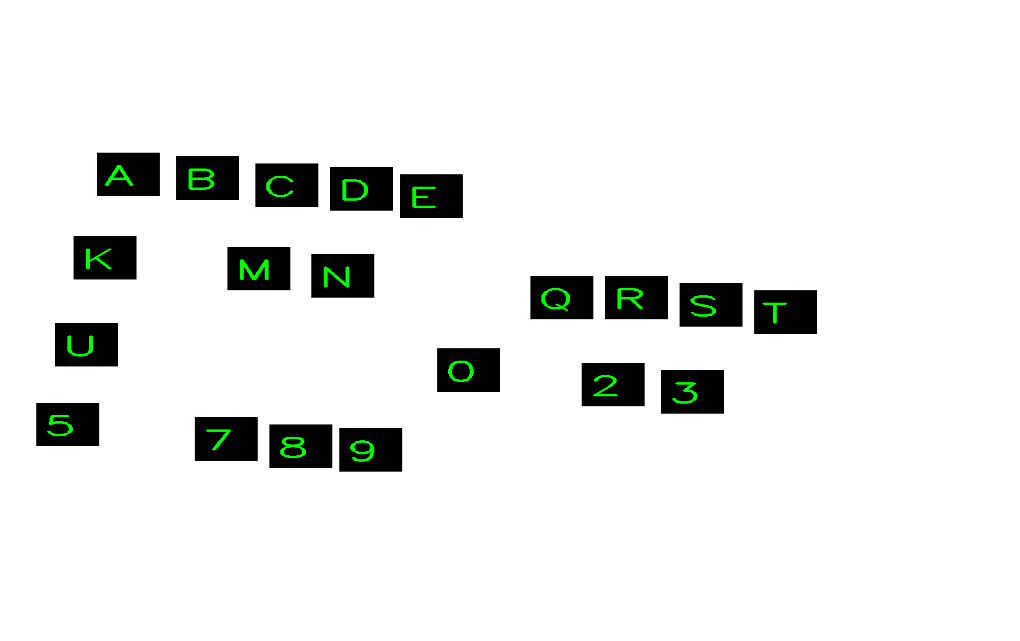
\includegraphics[scale=0.5]{im7fail2}
	\caption{Result after classifier 2 has been applied to a rotated version of test image 1}
	\label{im7fail3}
\end{figure}

An other situation when the system fail is when the image containing the characters is a bit tilted. In this case the characters will no longer appear to have the same size. In figure \ref{im7fail5} and \ref{im7fail4} are the results when testing on a tilted version of figure \ref{im7}.

\begin{figure}[H]
\centering
	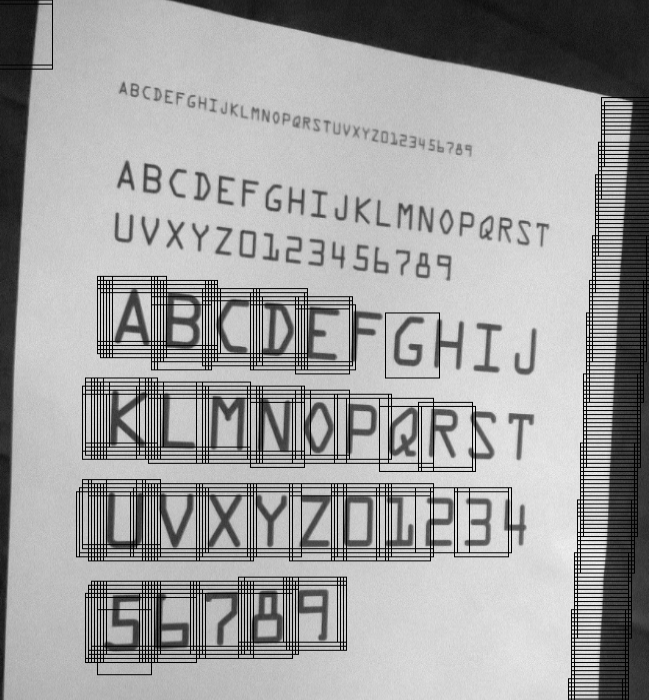
\includegraphics[scale=0.5]{im7fail5}
	\caption{Result after classifier 1 has been applied to a tilted version of test image 1}
	\label{im7fail5}
\end{figure}

\begin{figure}[H]
\centering
	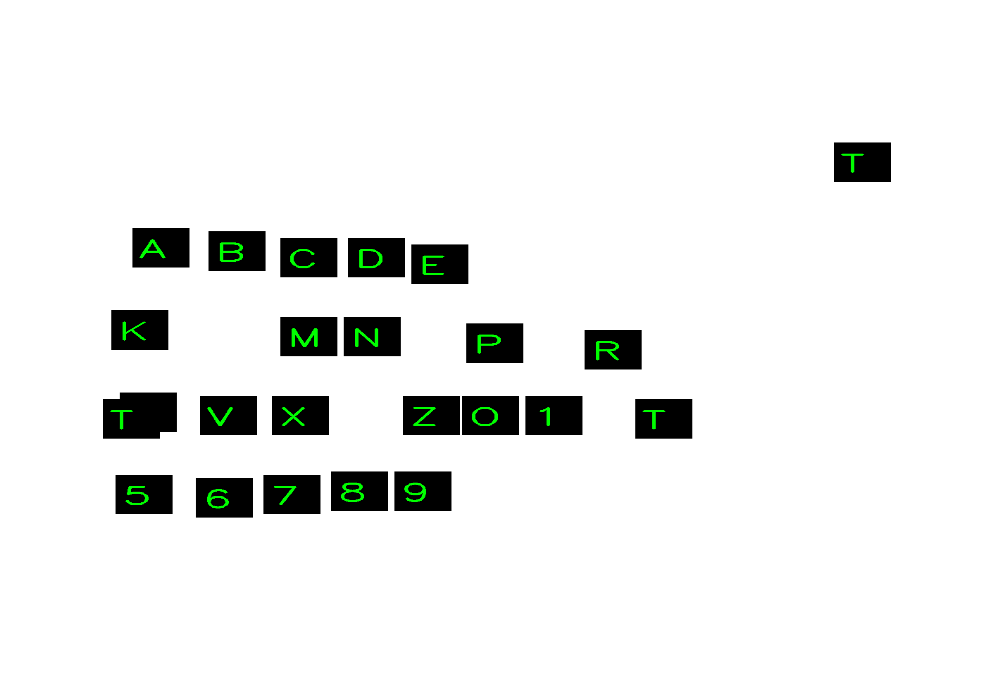
\includegraphics[scale=0.5]{im7fail4}
	\caption{Result after classifier 2 has been applied to a tilted version of test image 1}
	\label{im7fail4}
\end{figure}


\section{Comparison with two-rectangle features}
\label{sec:Comparison with two-rectangle features}
The two-rectangle features described in \ref{} is a type of haar-features which are commonly used as features in Random forest. For that reason it is of interest to make a comparison between the point pair features and the two-rectangle features. It is a rather difficult task since the amount of rectangles can be chosen arbitrarily. 

The comparison has been done by using the same training settings as was used in section \ref{sec:Evaluation of training} for training with point pair features with 4100 training data. Here the number of filters varies instead of the number of point pairs. The number of filters varies by increasing the amount of different filter sizes by starting with one filter of size 54x54 and then adding smaller filters.

\begin{table}[H]
\begin{center}
     \begin{tabular}{| l | l | l | l | l | l | }
     \hline
     features & 1 tree & 20 trees & 50 trees & 100 trees & 500 trees \\ \hline
     68 & 17 & 36 & 45 & 45 & 53 	\\ \hline
   	 170 & 16 & 34 & 45 & 46 & 50 	\\ \hline
     306 & 17 & 37 & 47  & 51  & 53	\\ \hline
     476 & 19 & 39 & 47 & 50 & 57	\\ \hline
     680 & 19 & 42 & 49 & 55 & 60	\\ \hline
	 1020 & 20 & 42 & 53 & 58 & 63	\\ \hline
	 1428 & 21 & 48 & 59 & 64 & 71	\\ \hline
	 2142 & 16 & 40 & 55 & 58 & 68	\\ \hline
	 3179 & 15 & 42 & 54 & 62 & 67	\\ \hline
	 4998 & 22 & 42 & 52 & 55 & 67	\\ \hline
	 7956 & 18 & 44 & 54 & 59 & 67	\\ \hline
     \end{tabular}
\end{center}
\caption{The amount of true detection in percent for classifier trained with different number of trees and different amount of training data}
\end{table}

\begin{table}[H]
\begin{center}
     \begin{tabular}{| l | l | l | l | l | l | }
     \hline
     features & 1 tree & 20 trees & 50 trees & 100 trees & 500 trees \\ \hline
     68 & 0.095 & 0.12 & 0.16 & 0.18 & 0.74	\\ \hline
   	 170 & 0.16 & 0.21 & 0.26 & 0.23 & 0.82 	\\ \hline
     306 & 0.22 & 0.33 & 0.35 & 0.33 & 0.92	\\ \hline
     476 & 0.30 & 0.44 & 0.49 & 0.46 & 1.04 	\\ \hline
     680 & 0.42 & 0.58 & 0.56 & 0.49 & 1.14	\\ \hline
	 1020 & 0.8 & 0.62 & 0.72 & 0.68 & 1.25	\\ \hline
	 1428 & 0.64 & 0.77 & 0.94 & 0.82 & 1.43	\\ \hline
	 2142 & 0.86 & 1.07 & 1.22 & 1.04 & 1.70	\\ \hline
	 3179 & 1.04 & 1.43 & 1.41 & 1.34 & 1.92	\\ \hline
	 4998 & 1.45 & 1.75 & 2.06 & 1.59 & 2.32	\\ \hline
	 7956 & 2.05 & 2.7 & 2.31 & 2.10 & 2.91	\\ \hline
     \end{tabular}
\end{center}
\caption{The amount of true detection in percent for classifier trained with different numbers of point pairs and different amount of trees using 4100 training data}
\end{table}

\section{Conclusions}
\label{sec:Conclusions}
When training the classifier with different number of point pairs the result does not seem to get better with more than 500 point pairs. Also there is no improvement when increasing the number of trees from 100 to 500. However the average time for each character increases a lot with more trees. Consequently, the number of trees should not be more than necessary if the purpose is to make a fast system. The number of point pairs doesn't seem to affect the time as much as the number of trees.
 
One thing that increases the performance a lot for both classifiers is the amount of training data. When increasing the amount of training data the time to train the classifier increases. However the time during testing stays the same. For that reason there is no concern if the training data is too much. 

With the current training data the image has to be viewed more or less exactly from above. If the image is viewed more from the side which was tested in figure, the result will be bad. The reason for this is that the characters have no longer the same size. It would be possible to include some train data where the characters are a bit smaller than the characters in sample images.

Also the angle of the characters in the training dataset has only changed between -5 and 5 degrees, hence the system will fail if the image is rotated too much. If it is desirable to make the system work for images that are rotated in some way the possible degree of rotation for the training samples has to be larger. However the amount of training data would then need to be bigger.

The system seems to fail when there are other characters in the images which are larger then the characters the system is drying to detect, see figure. This seems to be a very difficult case. The first classifier makes many false detections on the larger characters which leads to a lot of false predictions.

The system is a lot faster on images which is zoomed in on the area where the characters are. When the characters are large the tile will be large as well and this will make the total amount of tiles less. 